\subsection{Deployment view}
\par
Regarding the deployment, there are many quality to take into consideration. One of these is the scalability property: at the beginning 
TrackMe might only have few users, but once the usage is increasing more and more, the system must continue to work even if the 
requests from the users are huge. To achieve this quality of service, TrackMe needs the help of cloud database providers. These ones 
are specialized in the management of big database; and in this case the Share Data Service require a huge database in order to store 
all the data collected from the users. 
\par
On the other side, services such as Account Service, Individual Request Service and Group Request Service do not require so much 
power. Therefore, a good solution is the virtualization; in such a way each microservices has its own application server, while 
the database server can be shared among these services.. Instead, Spectator Service require to save a good amount of data and 
the access might be frequent due to the requirement regarding the possibility to see all the positions of the runners during a race. 
Consequently, Spectator Service has its own database 
server machine.
\par
To access these microservices one needs to use the mobile application which has to be installed either on an Android device or on a iOS 
device; Firewalls are used to separate the client domain and the server domain, and also used to filter packets which can be malevolent.
\begin{figure}[H]
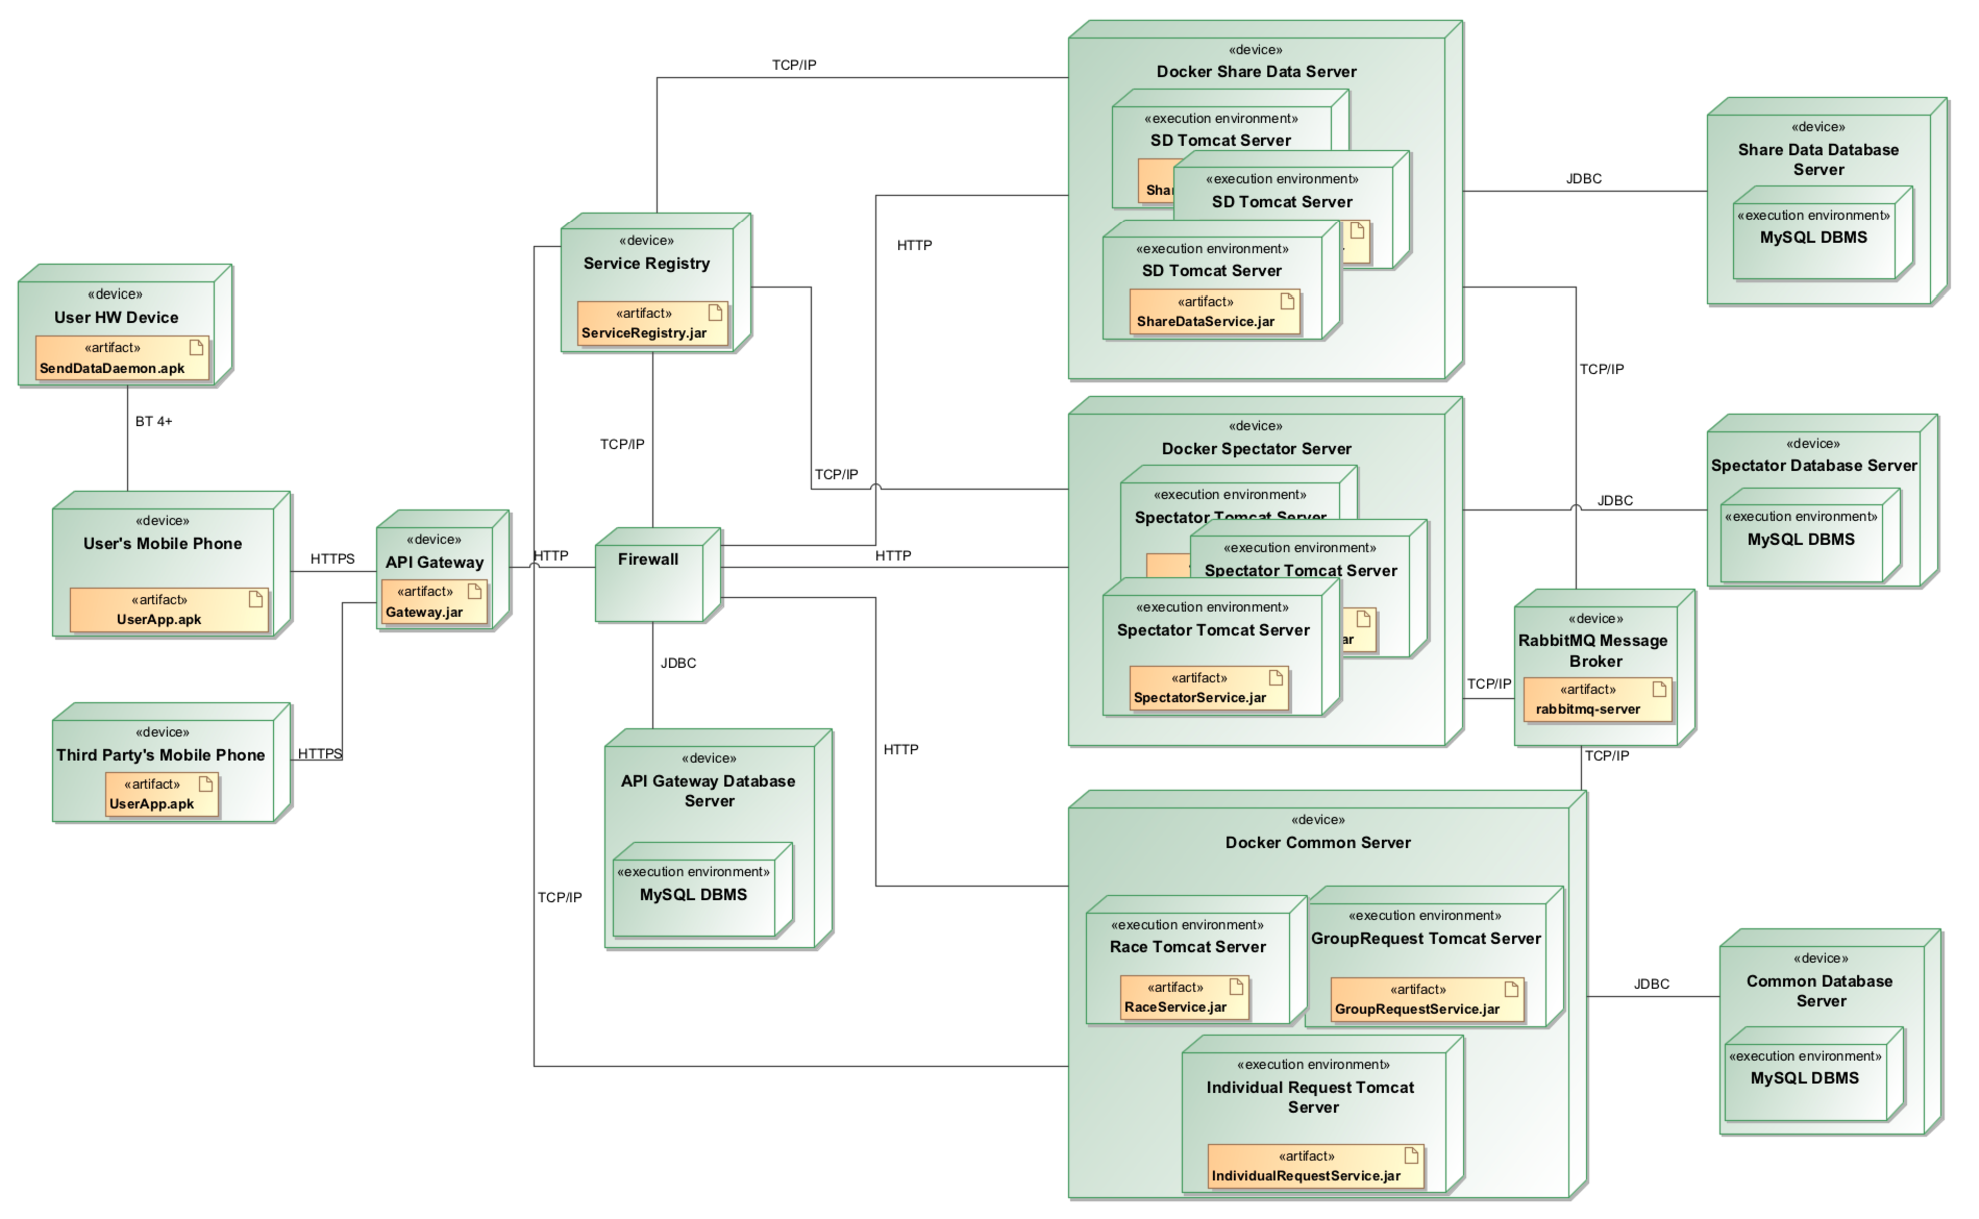
\includegraphics[width=\linewidth]{Images/deploymentdiagram.pdf}
\caption{ Deployment diagram with Archimate }
\label{fig:deployment}
\end{figure}
The deployment diagram represents the system to-be which is based on the microservices "reference architecture". Even if 
microservices offer the possibility to implement different services with different programming language or framework, what is simpler 
is to keep using the same environment. In this case, Glassfish application server and Oracle DBMS are strongly used. In conclusion, 
the system can be also seen as clients and many servers with 4 tier:
\begin{itemize}
\item Tier 1: Client side, which is the presentation
\item Tier 2: API Gateway, which redirects all the requests from the client to the respective application server
\item Tier 3: Application servers, which contains the logic business of the system
\item Tier 4: Database servers, in which it contains all the data
\end{itemize}